\input{preamble.tex}
\usepackage{eurosym} % pour le symbole euro propre

\begin{document}

\reversemarginpar

\pagestyle{fancy}
\fancyhead[L]{Terminale STMG}
\fancyhead[C]{\textbf{DS n°6a - Statistiques à deux variables}}
\fancyhead[R]{\today}

\null\vspace{-30pt}
Nom / Prénom : \\

Consignes particulières : 
\begin{itemize}[label=$\bullet$]
	\item 
	La calculatrice est {autorisée}.
	\item 
	Toute trace de recherche est prise en compte.
\end{itemize}

\hrule

\exe{10}{
Une entreprise étudie les variations de ses ventes (variable $y$) en fonction du prix unitaire de son produit (variable $x$). 
Les données sont présentées dans le tableau ci-dessous :
 \begin{center}
  \begin{tabular}{|l|*8{c|}}
	 \hline
	 \textbf{Prix : $x_i$} & 40 & 50 & 80 & 90 & 100 & 120 & 140 & 170 \\
	 \hline
	 \textbf{Nombre ventes : $y_i$} & 238 & 227 & 185 & 167 & 140 & 119 & 87 & 48 \\
	 \hline
	\end{tabular}
 \end{center}
 
On a représenté dans le repère ci-dessous le nuage de points associé à cette série statistique à deux variables :
  
\begin{tikzpicture}
\begin{axis}%
    [
        grid=major,  
        x=1mm,
        y=0.6mm,
        xtick={40,50,...,170},   
        xmin=40,
        xmax=180,
        xlabel={\small $x$},
        axis x line=middle,
        ytick={40,50,...,240},
        tick label style={font=\small},
        ymin=40,
        ymax=250,
        ylabel={\small $y$},
        axis y line=middle,
        no markers,
        samples=100,
    ]
\addplot[teal, only marks] 
table[x=x,y=y, col sep=comma] {data_DS6a1.csv};
\end{axis}
\end{tikzpicture}

\begin{enumerate}
  \item Calculer les coordonnées du point moyen G de ce nuage de points. Placer G sur le graphique.
  \item \begin{enumerate}
	 \item Justifier qu'il est pertinent de réaliser un ajustement affine pour ce nuage de points.
	 \item Déterminer une équation de la droite $\Delta$ d'ajustement affine de $y$ en $x$ obtenue par la méthode des moindres carrés, sous la forme $y=ax+b$.
	 On arrondira les paramètres à $10^{-1}$ près.
	\end{enumerate}
	\item Vérifier que la droite $\Delta$ passe par G.
	\item À l'aide de cet ajustement affine, estimer le nombre de ventes pour un prix unitaire de 150 \euro.
	\item Selon vous, quel est le prix permettant à l'entreprise de réaliser le plus grand chiffre d'affaire ?
 \end{enumerate}
}{exe:1a}{
\begin{enumerate}
  \item $G(\bar{x}, \bar{y})$ soit $G(98,75 ; 151,875)$.
  \item \begin{enumerate}
	 \item Les points présentent une tendance linéaire.
	 \item On trouve $a \approx -1,5$ et $b \approx 299,8$.
	\end{enumerate}
	\item Par définition, $b = \bar{y} - a \bar{x}$ donc, pour $x = \bar{x}$, l'ordonnée correspondante est 
	\begin{align*}
	y & = a \bar{x} + b \\
	& = a \bar{x} + \bar{y} - a \bar{x} \\
	& = \bar{y} .
	\end{align*}
	Donc la droite $(\Delta)$ passe par $G(\bar{x}, \bar{y})$.
	\item Pour $x = 150$ on trouve $y \approx 74$.
	\item Le chiffre d'affaire est donné par $CA(x) = x \times y \approx x(ax+b)$ avec $a \approx -1,5$ et $b \approx 299,8$.
	On veut donc maximiser la fonction $CA(x) = -1,5x^2 + 299,8 x$ sur $[0, \infty[$. \\
	On dérive : $CA'(x) = -3x + 299,8$, la dérivée s'annule pour $x \approx 100$, on peut maintenant dresser le tableau :

	\begin{center}
		\begin{tikzpicture}
		   \tkzTabInit{$x$ / 1 , $CA'(x)$ / 1, $CA(x)$ / 1.5}{$0$, $100$, $\infty$}
		   \tkzTabLine{, +, z, -,}
		   \tkzTabVar{-/ , +/, -/ }
		\end{tikzpicture}
	\end{center}
	
	La fonction atteint donc un maximum pour $x \approx 100$ ce qui correspond à un chiffre d'affaire :
	\begin{align*}
	CA(100) & \approx -1.5 \times (100)^2 + 299,8 \times 100  \\
	& \approx 14~980 \\
	\end{align*}
	Soit 14~980 \euro~pour un prix unitaire de 100 \euro.
 \end{enumerate}
}

\exe{10}{
Un gel antibactérien est testé en laboratoire. Pour un volume donné de gel (variable $v$, en mililitres), les scientifiques observent
le pourcentage de bactéries éliminées (variable $y$, appelée efficacité).

Les données sont compilées dans le tableau ci-dessous :

 \begin{center}
  \begin{tabular}{|l|*8{c|}}
	 \hline
	 \textbf{Volume : $v_i$} & 0,4 & 0,8 & 1,4 & 2,5 & 4,5 & 6 & 7,9 & 10,6 \\
	 \hline
	 \textbf{Efficacité : $y_i$} & 40 & 50 & 60 & 70 & 80 & 85 & 90 & 95 \\
	 \hline
	\end{tabular}
 \end{center}
 
Le nuage de points correspondant est donné ci-dessous :
\begin{center}
 \begin{tikzpicture}
\begin{axis}%
    [
        grid=major,  
        x=10mm,
        y=2mm,
        xtick={0,1,...,11},   
        xmin=0,
        xmax=11,
        xlabel={\small $v$},
        axis x line=middle,
        ytick={40,45,...,95},
        tick label style={font=\small},
        ymin=40,
        ymax=100,
        ylabel={\small $y$},
        axis y line=middle,
        no markers,
        samples=100,
    ]
\addplot[teal, only marks] 
table[x=x,y=y, col sep=comma] {data_DS6a2.csv};
\end{axis}
\end{tikzpicture}
\end{center}
\begin{enumerate}
\item Un ajustement affine du nuage de points vous semble-t-il pertinent ? Justifier.
\item On propose de réaliser une transformation logarithmique de la variable $v$ de volume en posant $x_i = \log(v_i)$.
Compléter le tableau ci-dessous en arrondissant $x_i$ à $10^{-1}$ près.
 \begin{center}
  \begin{tabular}{|l|*8{c|}}
	 \hline
	 \textbf{$x_i = \log(v_i)$} & \dots & \dots & \dots & \dots & \dots & \dots & \dots & \dots \\
	 \hline
	 \textbf{Efficacité : $y_i$} & 40 & 50 & 60 & 70 & 80 & 85 & 90 & 95 \\
	 \hline
	\end{tabular}
 \end{center}
\item Représenter le nouveau nuage de points $M_i(x_i,y_i)$ dans un repère orthogonal. \\
\textit{Conseil : en abscisse, utilisez 1 cm pour une variation de 0,1 unité et en ordonnée, 1 cm pour une variation de 5 \% .}
\item Calculer les coordonnées du point moyen G de ce nuage de points et placer le sur le graphique.
\item Déterminer une équation de la droite $\Delta$ d'ajustement affine de $y$ en $x$ obtenue par la méthode des moindres carrés,
sous la forme $y=ax+b$. On arrondira les paramètres à $10^{-1}$ près. Tracer cette droite dans le repère.
\item Estimer le pourcentage (arrondi à $10^{-1}$ près) de bactéries éliminées si on utilise 14 mililitres de gel antibactérien.
\end{enumerate}
}{exe:2a}{

\begin{enumerate}
\item Non, les points ne présentent pas de tendance linéaire.
\item ~\\
 \begin{center}
  \begin{tabular}{|l|*8{c|}}
	 \hline
	 \textbf{$x_i = \log(v_i)$} & -0,4 & -0,1 & 0,1 & 0,4 & 0,7 & 0,8 & 0,9 & 1 \\
	 \hline
	 \textbf{Efficacité : $y_i$} & 40 & 50 & 60 & 70 & 80 & 85 & 90 & 95 \\
	 \hline
	\end{tabular}
 \end{center}
\item 

\begin{center}
\begin{tikzpicture}
\begin{axis}
    [
        grid=major,  
        x=80mm,
        y=1mm,
        xtick={-0.4,-0.3,...,1},   
        xmin=-0.4,
        xmax=1.1,
        xlabel={\small $x$},
        axis x line=middle,
        ytick={40,45,...,95},
        tick label style={font=\small},
        ymin=40,
        ymax=100,
        ylabel={\small $y$},
        axis y line=middle,
        no markers,
        samples=100,
    ]
\addplot[teal, only marks] 
table[x=x,y=y, col sep=comma] {data_DS6a2_correc.csv};
\end{axis}
\end{tikzpicture}
\end{center}

\item $G(0,425 ; 71,25)$.
\item On trouve $a \approx 38,6$ et $b \approx 54,9$.
\item Pour $v_9 = 14$, on a $x_9 = \log(p_9) \approx 1,1$ et en utilisant $y_9 \approx a x_9 + b$ on trouve une efficacité d'environ
97 \%.
\end{enumerate}
%FIN CORREC 2a
}

%%%%%%%%%%%%% SUJET B %%%%%%%%%%%%%%
\setcounter{Exercise}{0}

\newpage

\pagestyle{fancy}
\fancyhead[L]{Terminale STMG}
\fancyhead[C]{\textbf{DS n°6b - Statistiques à deux variables}}
\fancyhead[R]{\today}

\null\vspace{-30pt}
Nom / Prénom : \\

Consignes particulières : 
\begin{itemize}[label=$\bullet$]
	\item 
	La calculatrice est {autorisée}.
	\item 
	Toute trace de recherche est prise en compte.
\end{itemize}

\hrule

\exe{10}{
Une entreprise étudie les variations de ses ventes (variable $y$) en fonction du prix unitaire de son produit (variable $x$). 
Les données sont présentées dans le tableau ci-dessous :
 \begin{center}
  \begin{tabular}{|l|*8{c|}}
	 \hline
	 \textbf{Prix : $x_i$} & 60 & 70 & 80 & 100 & 110 & 120 & 130 & 150 \\
	 \hline
	 \textbf{Nombre ventes : $y_i$} & 248 & 223 & 202 & 147 & 120 & 102 & 73 & 26 \\
	 \hline
	\end{tabular}
 \end{center}
 
On a représenté dans le repère ci-dessous le nuage de points associé à cette série statistique à deux variables :
  
\begin{tikzpicture}
\begin{axis}%
    [
        grid=major,  
        x=1.4mm,
        y=0.5mm,
        xtick={60,70,...,150},   
        xmin=60,
        xmax=160,
        xlabel={\small $x$},
        axis x line=middle,
        ytick={20,30,...,250},
        tick label style={font=\small},
        ymin=20,
        ymax=250,
        ylabel={\small $y$},
        axis y line=middle,
        no markers,
        samples=100,
    ]
\addplot[teal, only marks] 
table[x=x,y=y, col sep=comma] {data_DS6b1.csv};
\end{axis}
\end{tikzpicture}

\begin{enumerate}
  \item Calculer les coordonnées du point moyen G de ce nuage de points. Placer G sur le graphique.
  \item \begin{enumerate}
	 \item Justifier qu'il est pertinent de réaliser un ajustement affine pour ce nuage de points.
	 \item Déterminer une équation de la droite $\Delta$ d'ajustement affine de $y$ en $x$ obtenue par la méthode des moindres carrés, sous la forme $y=ax+b$.
	 On arrondira les paramètres à $10^{-1}$ près.
	\end{enumerate}
	\item Vérifier que la droite $\Delta$ passe par G.
	\item À l'aide de cet ajustement affine, estimer le nombre de ventes pour un prix unitaire de 140 \euro.
	\item Selon vous, quel est le prix permettant à l'entreprise de réaliser le plus grand chiffre d'affaire ?
 \end{enumerate}
}{exe:1b}{
\begin{enumerate}
  \item $G(\bar{x}, \bar{y})$ soit $G(102,5 ; 142,625)$.
  \item \begin{enumerate}
	 \item Les points présentent une tendance linéaire.
	 \item On trouve $a \approx -2,5$ et $b \approx 397,3$.
	\end{enumerate}
	\item Par définition, $b = \bar{y} - a \bar{x}$ donc, pour $x = \bar{x}$, l'ordonnée correspondante est 
	\begin{align*}
	y & = a \bar{x} + b \\
	& = a \bar{x} + \bar{y} - a \bar{x} \\
	& = \bar{y} .
	\end{align*}
	Donc la droite $(\Delta)$ passe par $G(\bar{x}, \bar{y})$.
	\item Pour $x = 140$ on trouve $y \approx 49$.
	\item Le chiffre d'affaire est donné par $CA(x) = x \times y \approx x(ax+b)$ avec $a \approx -2,5$ et $b \approx 397,3$.
	On veut donc maximiser la fonction $CA(x) = -2,5x^2 + 397,3 x$ sur $[0, \infty[$. \\
	On dérive : $CA'(x) = -5x + 397,3$, la dérivée s'annule pour $x \approx 50$, on peut maintenant dresser le tableau :

	\begin{center}
		\begin{tikzpicture}
		   \tkzTabInit{$x$ / 1 , $CA'(x)$ / 1, $CA(x)$ / 1.5}{$0$, $50$, $\infty$}
		   \tkzTabLine{, +, z, -,}
		   \tkzTabVar{-/ , +/, -/ }
		\end{tikzpicture}
	\end{center}
	
	La fonction atteint donc un maximum pour $x \approx 50$ ce qui correspond à un chiffre d'affaire :
	\begin{align*}
	CA(50) & \approx -2.5 \times (50)^2 + 397,3 \times 50  \\
	& \approx 13~615 \\
	\end{align*}
	Soit 13~615 \euro~pour un prix unitaire de 50 \euro.
 \end{enumerate}
}

\exe{10}{
Un gel antibactérien est testé en laboratoire. Pour un volume donné de gel (variable $v$, en mililitres), les scientifiques observent
le pourcentage de bactéries éliminées (variable $y$, appelée efficacité).

Les données sont compilées dans le tableau ci-dessous :

 \begin{center}
  \begin{tabular}{|l|*8{c|}}
	 \hline
	 \textbf{Volume : $v_i$} & 0,5 & 0,9 & 1,6 & 2,7 & 4,8 & 6,4 & 8,4 & 11,2 \\
	 \hline
	 \textbf{Efficacité : $y_i$} & 40 & 50 & 60 & 70 & 80 & 85 & 90 & 95 \\
	 \hline
	\end{tabular}
 \end{center}
 
Le nuage de points correspondant est donné ci-dessous :
\begin{center}
 \begin{tikzpicture}
\begin{axis}%
    [
        grid=major,  
        x=10mm,
        y=2mm,
        xtick={0,1,...,11},   
        xmin=0,
        xmax=12,
        xlabel={\small $v$},
        axis x line=middle,
        ytick={40,45,...,95},
        tick label style={font=\small},
        ymin=40,
        ymax=100,
        ylabel={\small $y$},
        axis y line=middle,
        no markers,
        samples=100,
    ]
\addplot[teal, only marks] 
table[x=x,y=y, col sep=comma] {data_DS6a2.csv};
\end{axis}
\end{tikzpicture}
\end{center}
\begin{enumerate}
\item Un ajustement affine du nuage de points vous semble-t-il pertinent ? Justifier.
\item On propose de réaliser une transformation logarithmique de la variable $v$ de volume en posant $x_i = \log(v_i)$.
Compléter le tableau ci-dessous en arrondissant $x_i$ à $10^{-1}$ près.
 \begin{center}
  \begin{tabular}{|l|*8{c|}}
	 \hline
	 \textbf{$x_i = \log(v_i)$} & \dots & \dots & \dots & \dots & \dots & \dots & \dots & \dots \\
	 \hline
	 \textbf{Efficacité : $y_i$} 40 & 50 & 60 & 70 & 80 & 85 & 90 & 95 \\
	 \hline
	\end{tabular}
 \end{center}
\item Représenter le nouveau nuage de points $M_i(x_i,y_i)$ dans un repère orthogonal. \\
\textit{Conseil : en abscisse, utilisez 1 cm pour une variation de 0,1 unité et en ordonnée, 1 cm pour une variation de 5 \% .}
\item Calculer les coordonnées du point moyen G de ce nuage de points et placer le sur le graphique.
\item Déterminer une équation de la droite $\Delta$ d'ajustement affine de $y$ en $x$ obtenue par la méthode des moindres carrés,
sous la forme $y=ax+b$. On arrondira les paramètres à $10^{-1}$ près. Tracer cette droite dans le repère.
\item Estimer le pourcentage (arrondi à $10^{-1}$ près) de bactéries éliminées si on utilise 14 mililitres de gel antibactérien.
\end{enumerate}
}{exe:2b}{

\begin{enumerate}
\item Non, les points ne présentent pas de tendance linéaire.
\item ~\\
 \begin{center}
  \begin{tabular}{|l|*8{c|}}
	 \hline
	 \textbf{$x_i = \log(v_i)$} & -0,4 & -0,1 & 0,1 & 0,4 & 0,7 & 0,8 & 0,9 & 1 \\
	 \hline
	 \textbf{Efficacité : $y_i$} & 40 & 50 & 60 & 70 & 80 & 85 & 90 & 95 \\
	 \hline
	\end{tabular}
 \end{center}
\item 

\begin{center}
\begin{tikzpicture}
\begin{axis}
    [
        grid=major,  
        x=80mm,
        y=1mm,
        xtick={-0.3,-0.2,...,1},   
        xmin=-0.3,
        xmax=1.1,
        xlabel={\small $x$},
        axis x line=middle,
        ytick={40,45,...,95},
        tick label style={font=\small},
        ymin=40,
        ymax=100,
        ylabel={\small $y$},
        axis y line=middle,
        no markers,
        samples=100,
    ]
\addplot[teal, only marks] 
table[x=x,y=y, col sep=comma] {data_DS6b2_correc.csv};
\end{axis}
\end{tikzpicture}
\end{center}

\item $G(0,4625 ; 71,25)$.
\item On trouve $a \approx 42,4$ et $b \approx 51,6$.
\item Pour $v_9 = 14$, on a $x_9 = \log(p_9) \approx 1,1$ et en utilisant $y_9 \approx a x_9 + b$ on trouve une efficacité d'environ 
98 \%.
\end{enumerate}

}


%%%%%%%%%%%%

\newpage
\fancyhead[C]{\textbf{Solutions}}
Les solutions sont données dans l'ordre sujet a puis b. \newline
\shipoutAnswer


\end{document}
